\section{Objectives}
By the end of this lab work, students are expected to learn how to 

\begin{itemize}
\item operate a function generator,
\item operate an oscilloscope,
  
\item measure the period and frequency of a sine wave using an oscilloscope, and 
  
\item measure rise time, fall time, pulse width, and duty cycle of a pulse waveform using an oscilloscope.
  

\end{itemize}

\section{Parts}
\label{sec:partsEx5}

\begin{enumerate}
\item Breadboard    
\item One $2.7~[\kilo\ohm]$ resistor, 
\item One $6.8~[\kilo\ohm]$ resistor, and 
  
\item One $1000~[\pico\farad]$ capacitor. 
\end{enumerate}

\section{Background}
\label{sec:background}

This laboratory assignment deals with alternating voltages and currents (AC)
that vary with respect to time. The constructed circuit will be powered from an
AC voltage source. For simplicity, you will be using an AC voltage source that
provides a time-varying periodic voltage (function of time) which is mathematically represented
as %
%
\begin{align*}
  v(t) = v(t+T),
\end{align*}
%
where $v(t)$ is the voltage at time $t\ge 0$ and $T$ is the time period at which
the voltage (or any signal in general), $v(t),$ repeats itself. Therefore, the
signal $v(t)$ can be represented in the form of a wave. The most common
waveforms that you will be using throughout this course and laboratory
assignments are: %
%
\begin{itemize}
\item sine,
  
\item square,
  
\item pulse, and
  
\item triangular
\end{itemize}
%
waveforms. In general, a signal $v(t)$ that forms a sine wave is defined by %
%
\begin{align*}
  v(t) = a\cdot\sin(\omega\cdot t)  = a\cdot\sin(\frac{2\pi}{T}t),
\end{align*}
where $a$ is the amplitude of the signal $v(t)$. Figure~\ref{fig:figure1-sinWave} shows the sine waveform of a voltage signal with its amplitude $a~[\volt]$ (peak-to-peak amplitude $V_{\text{pp}} = 2a).$ The \emph{period} $T$ is the time difference between two points on the waveform where the signal $v(t)$ repeats. The frequency of the signal $v(t)$ is $f,$ where $f = \frac{1}{T}.$ The AC signal $v(t)$ can also be represented as a phasor quantity. Recall that a phasor is a complex number used to represent a sinusoidal signal using its amplitude and phase. The phasor of a cosinusoidal signal of the form $v_1(t) = V_1\cos(\omega t + \theta_1)$ is given by ${\bf V}_1 = V_1\angle{\theta_1}.$ If the signal is a sinusoid of the form $v_2(t) =V_2\sin(\omega t +\theta_2),$ we first convert the signal using the trigonometric identity $\sin(z) = \cos(z-90^{\degree}).$ Therefore, we have $v_2(t) =V_2\sin(\omega t +\theta_2) = V_2\cos(\omega t +\theta_2 - 90^{\degree})$ and its phasor is ${\bf V}_2 = V_2\angle{(\theta_2-90^{\degree})}.$ 

\begin{figure}
    \centering
    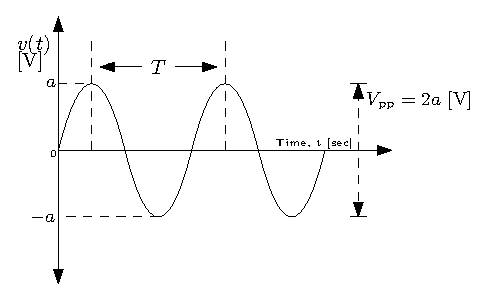
\includegraphics[width=0.5\textwidth]{figs/ipe/lab5/figure1-sinWave.eps}
    \caption{A sinusoidal (sine) waveform with a phase of $0^{\degree}.$}
    \label{fig:figure1-sinWave}
\end{figure}

The square wave of a signal $v(t)$ with amplitude $a$ is described  mathematically by %
%
\begin{align*}
  v(t) = a\cdot\text{sign}(\sin(\omega t)),
\end{align*}
%
where the operator $\text{sign}(\cdot)$ is defined as %
\begin{align*}
  \text{sign}(\sin(\omega t)) = 
  \begin{cases}
    1 & \text{if}~~\sin(\omega t)\ge 0,\\
    -1 & \text{otherwise.}
  \end{cases}
\end{align*}
%
Figure~\ref{fig:figure2-squareWave} shows a square waveform with amplitude $a$ and period $T.$ 

    \begin{figure}
        \centering
        \begin{tikzpicture}
          \draw[step=\smgrid,gray,ultra thin] 
          (0,-7*\smgrid) grid (25*\smgrid,7*\smgrid);
          % y-axis
          \draw[<->,ultra thick]
          (0,-7*\smgrid) -- (0,7*\smgrid)node[anchor=east]{$v(t)$};
          % x-axis
          \draw[->,ultra thick]
          (0,0)node[left]{$0$} -- (25*\smgrid,0)node[very near end, below]{Time, $t~[\second]$};
          % square wave 
          \draw[very thick,blue]
          (0,5*\smgrid)node[left]{$a$}--++(4*\smgrid,0) --++(0,-10*\smgrid)--++(4*\smgrid,0)--++(0,10*\smgrid)--++(4*\smgrid,0) --++(0,-10*\smgrid)--++(4*\smgrid,0)--++(0,10*\smgrid)--++(4*\smgrid,0) --++(0,-10*\smgrid)--++(4*\smgrid,0);
          \draw
          (0,-5*\smgrid)node[left]{$-a$};
          % period
          \draw[<->,>=stealth,thick,red]
          (4*\smgrid,6*\smgrid) --node[midway,above]{$T$}++(8*\smgrid,0);
          % Peak-to-peak amplitude
          \draw[<->,>=stealth,ultra thick,red,dashed]
          (10*\smgrid,-5*\smgrid) -- node[near end,below,rotate=90]{$V_{\text{pp}}=2a$}++(0,10*\smgrid);
        \end{tikzpicture}
        % 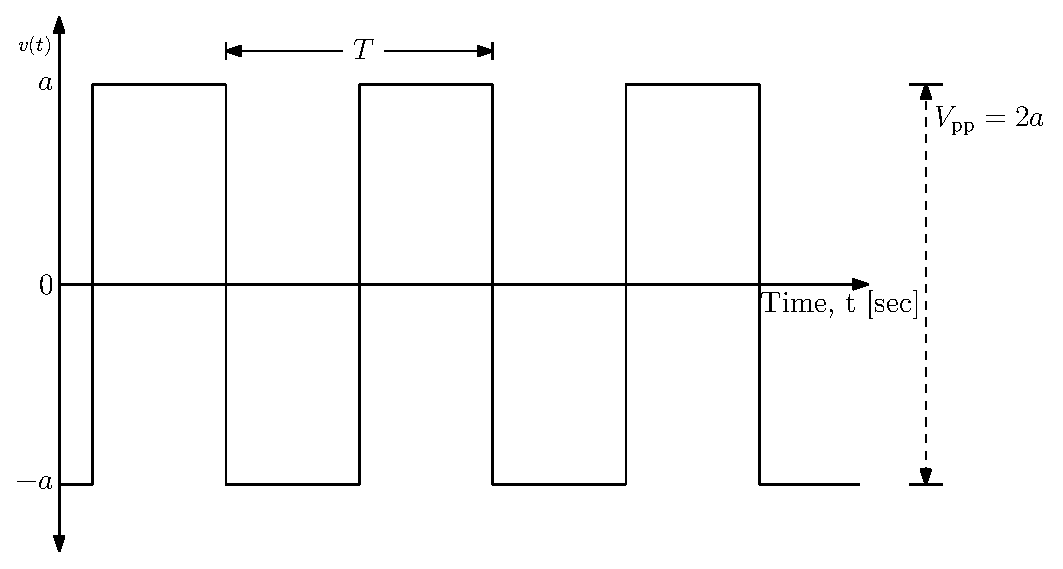
\includegraphics[width=0.55\textwidth]{figs/ipe/lab5/figure2-squareWave.eps}
        \caption{A square wave.}
        \label{fig:figure2-squareWave}
    \end{figure}
%

    \begin{figure}
    \centering
        \begin{tikzpicture}
          \draw[step=\smgrid,gray,ultra thin] 
          (0,0) grid (25*\smgrid,7*\smgrid);
          % y-axis
          \draw[->,ultra thick]
          (0,0) -- (0,7*\smgrid)node[anchor=east]{$v(t)$};
          % x-axis
          \draw[->,ultra thick]
          (0,0)node[left]{$0$} -- (25*\smgrid,0)node[very near end, below]{Time, $t~[\second]$};
          % pulse wave 
          \draw[very thick,blue]
          (0,5*\smgrid)node[left]{$a$}--++(4*\smgrid,0) --++(0,-5*\smgrid)--++(4*\smgrid,0)--++(0,5*\smgrid)--++(4*\smgrid,0) --++(0,-5*\smgrid)--++(4*\smgrid,0)--++(0,5*\smgrid)--++(4*\smgrid,0) --++(0,-5*\smgrid)--++(4*\smgrid,0);
          % Period
          \draw[<->,>=stealth,thick,red]
          (4*\smgrid,6*\smgrid) --node[midway,above]{$T$}++(8*\smgrid,0);
          % OFF time
          \draw[<->,>=stealth,thick,red,dashed]
          (4*\smgrid,\smgrid) --node[midway,above]{$T_{\text{off}}$}++(4*\smgrid,0);
          % ON time
          \draw[<->,>=stealth,thick,red,dashed]
          (8*\smgrid,2*\smgrid) --node[midway,above]{$T_{\text{on}}$}++(4*\smgrid,0);
          % Peak amplitude
          \draw[<->,>=stealth,ultra thick,red,dashed]
          (14*\smgrid,0) -- node[near end,below,rotate=90]{$V_{\text{p}}=a$}++(0,5*\smgrid);
        \end{tikzpicture}
    % 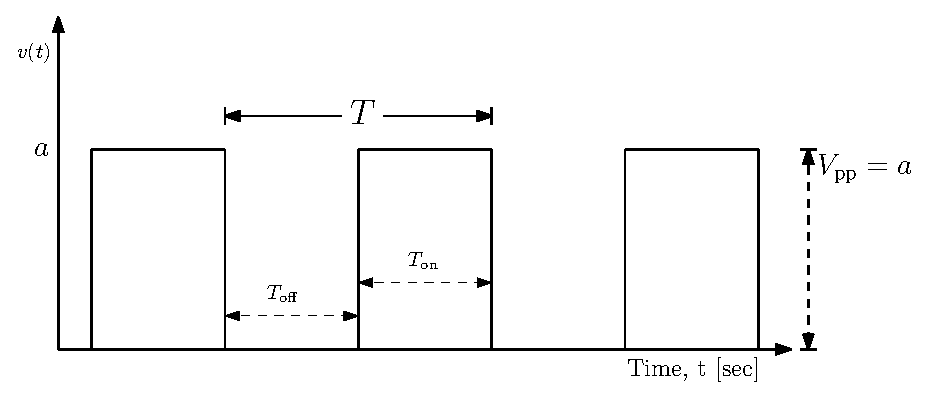
\includegraphics[width=0.55\textwidth]{figs/ipe/lab5/figure3a-idealPulse.eps}
    \caption{An ideal pulse wave.}
    \label{fig:figure3a-idealPulse}
    \end{figure}    
%
Without loss of generality, we define a pulse waveform as a special case of a square waveform with the negative amplitude set to  zero. Figure~\ref{fig:figure3a-idealPulse} depicts a pulse waveform showing its period and amplitude. The width of the pulse is defined by the duty cycle which is expressed in percentage as %
%
\begin{align*}
  \text{Duty cycle} (\%)  = \frac{T_{\text{on}}}{T} \times 100\%   = \frac{T_{\text{on}}}{T_{\text{on}} + T_{\text{off}}} \times 100\%,  
\end{align*}
%
where $T_{\text{on}}$ and $T_{\text{off}}$ denote the times when the pulse (signal) is \emph{on} and \emph{off}, respectively. A pulse waveform with a variable duty cycle is also called a pulse-width modulated (PWM)  waveform. Figure~\ref{fig:figure3a-idealPulse} shows the ideal pulse train of a signal.  However, the actual pulse train generated from a circuit may differ from the ideal case. The performance of an actual pulse is determined by the performance metrics \emph{rise time,} \emph{fall time,} \emph{overshoot,} and \emph{undershoot.} Figure~\ref{fig:figure3b-waveProperties} shows the performance metrics of a pulse. The time required for a pulse to rise (fall) from $10\%(90\%)$ to $90\%(10\%)$ is the \emph{rise(fall) time}.  The \emph{overshoot} and \emph{undershoot}  are shown in Figure~\ref{fig:figure3b-waveProperties} but descriptions of these performance metrics are omitted here for conciseness. %
%
    \begin{figure}
    \centering
    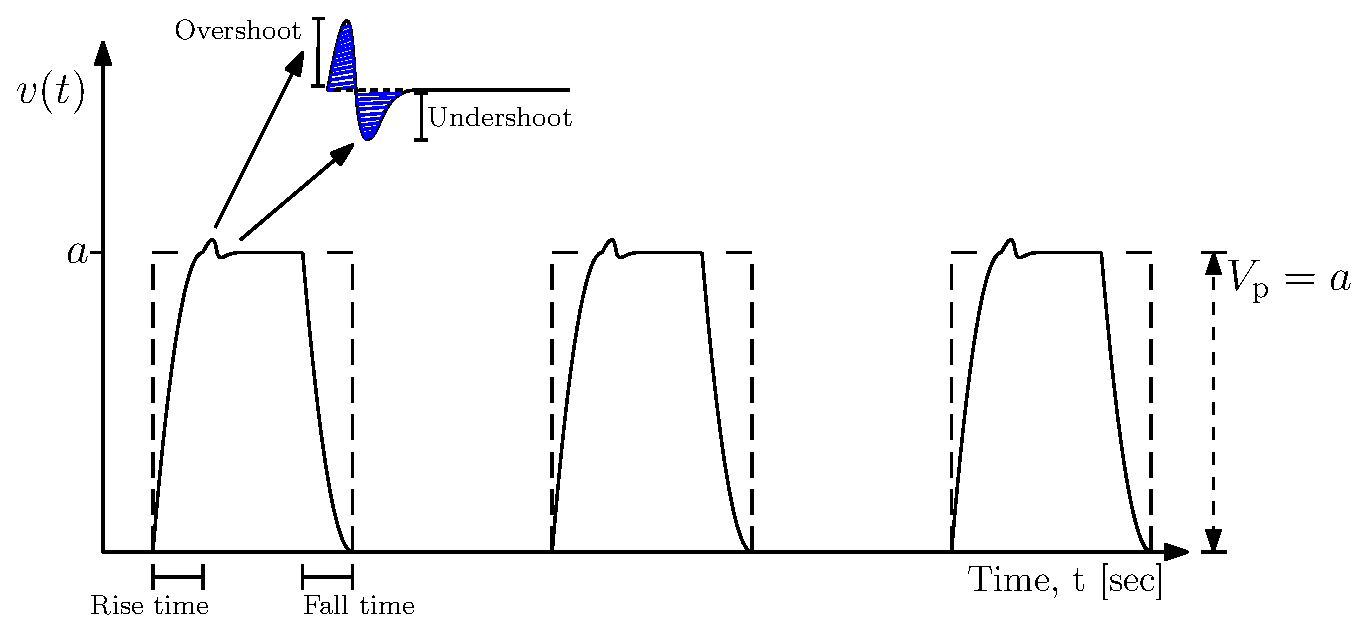
\includegraphics[width=0.5\textwidth]{figs/ipe/lab5/figure3b-waveProperties.eps}
    \caption{Actual pulse waveform}
    \label{fig:figure3b-waveProperties}    
    \end{figure}
%
We will not be working with triangular waveforms in this laboratory assignment, so the description of a triangular waveform is also omitted. The AC voltage in the form of sine, pulse, and triangular waveforms can be generated from the function generator provided at the laboratory workstation. These waveforms can also be observed/measured using a device called an oscilloscope. Before illustrating the task of this laboratory assignment, let us briefly introduce these devices in the next section. 


\section{AC Signal Generation and Measuring Equipment}
\label{sec:equipment}

In addition to the DC power supplies and the digital multimeters that were used in the previous laboratory experiments, you will be using two additional pieces of equipment which are mainly used to generate and measure AC signals. Two pieces of equipment that will be used in this lab assignment are:
\begin{enumerate}
    \item Function generator and 
    \item Oscilloscope. 
\end{enumerate}
%

\subsection{Function Generator}
\label{sec:functionGenerator}
The function generator provided at the laboratory workstation is shown in Figure~\ref{fig:Agilent33210A-FunctionGenerator}. This instrument will output desired voltage waveforms (AC voltage) with a frequency range of approximately $1~[\si{\hertz}]$ to $10~[\mega\hertz].$ It can produce ramp, triangle, pulse, sine, and square waveform outputs as well as allow for generating amplitude modulation, frequency modulation, and PWM signals. % %
% \todo[inline]{Annotate Function Generator}
\begin{figure}
    \centering
    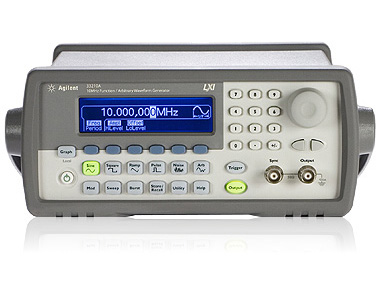
\includegraphics[width=0.5\textwidth]{figs/img/labs/Agilent33210A-FunctionGenerator.jpg}
    \caption{Agilent function generator used in the laboratory.}
    \label{fig:Agilent33210A-FunctionGenerator}
  \end{figure}
%  
Before you start using the function generator provided at the laboratory workstations, make sure to choose the following setup: 

\begin{itemize}
    \item \emph{Utility}$\rightarrow$ \emph{Output Setup} $\rightarrow$ \emph{High Z} $\rightarrow$ \emph{Done}
    \item \emph{Output} (turns ON the output waveform) 
\end{itemize}


\subsection{Oscilloscope}
\label{sec:oscilloscope}
The oscilloscope (``scope'' for short) is an instrument that is used to
graphically display the signal (voltage) of a circuit as a function of time. The
Tektronix TDS 2024B Oscilloscopes, for instance, provided at the laboratory
workstations have four channels. A channel can be used to measure and display
signals (for example, the voltage across a circuit element) on the screen of an
oscilloscope. Each channel of a scope contains a probe with a positive and
negative (ground) connections. Figure~\ref{fig:annotatedScope} shows the
Tektronix TDS 2024B oscilloscope with some basic functions annotated with text
arrows. However, you are encouraged to read the user manual of this
oscilloscope provided by its manufacturer. %, which can be found in the link provided below. %

% \mbox{
% \url{http://docs-europe.electrocomponents.com/webdocs/04c6/0900766b804c6b7c.pdf}
% }

The horizontal or vertical parameters of the display can be adjusted via the
corresponding knobs to view a more useful waveform. Another important function
of a scope is its ability to set a ``trigger" for a channel. The scope's trigger
function is used to achieve clear, stable signal characterization, as it
synchronizes the horizontal sweep of the oscilloscope to the desired point on
the signal. The trigger control will enable you to stabilize repetitive
waveforms as well as capture single-shot waveforms. %
%
\begin{figure}
    \centering
    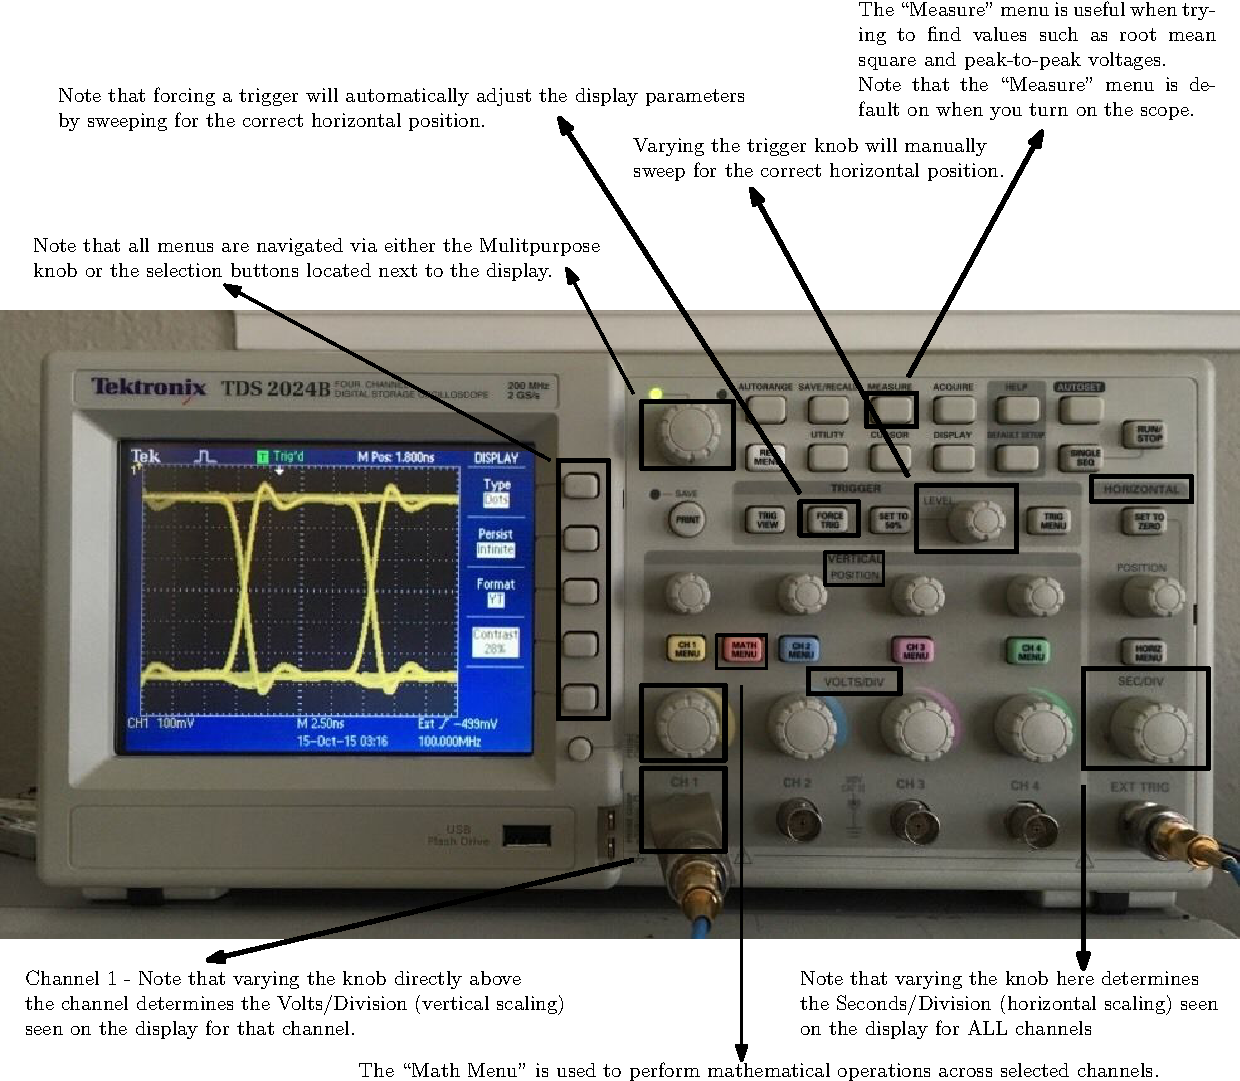
\includegraphics[width=0.7\textwidth]{figs/ipe/lab5/figure6-annotatedScope}
    \caption{Oscilloscope showing all basic functions.}
    \label{fig:annotatedScope}
\end{figure}


% \subsection{Part~1: Sine Wave}
% \label{sec:sineWave}


% \missingfigure{Figure 1: A sine wave showing its period and amplitude. }

% \missingfigure{Figure 2: A circuit with an AC voltage source (sine wave).}

% \subsection{Part~2: Pulse (Square) Waveform}
% \label{sec:voltageDivider}

% \missingfigure{Figure 1: An ideal square wave showing its period and amplitude. }

% \missingfigure{Figure 2: An actual square wave showing its rise time and fall time.}



\section{Prelab}
\label{sec:prelab}

The prelab for this lab assignment consists of two parts. In the first part, you are to determine the peak-voltage (amplitude), peak-to-peak voltage, angular frequency, frequency, and time period of a time-varying sinusoidal voltage. You will also need to determine its phasor representation. In the second part, you will convert the sinusoidal signal into a pulse waveform. For that, it is important that you familiarize yourself with unit step function, which is defined by %  
  %
  \begin{align}
    u(\alpha) =
    \begin{cases}
      1 & \text{for}~\alpha\ge 0,\\
      0 & \text{otherwise,}
    \end{cases}
    \label{eq:uAlpha}
  \end{align}
  %
  where $\alpha\in\mathbb{R}$ (\textit{i.e.,} $\alpha$ takes values from a set of real numbers). 

\begin{prelab}[Sine waveform]{prelab:sinewaveform}
  Suppose the voltage generated from a signal generator is given by %
  %
  \begin{align*}
    v(t) = 2\sin\left(\frac{44}{7}t\right) 
  \end{align*}
  %
  for time $t$ ranging from $0$ to $10~[\second].$ 
  \begin{enumerate}[(a)]
      \item Determine the peak-voltage $V_p$, peak-to-peak voltage $V_{\text{pp}},$ angular frequency $\omega,$ frequency  $f,$ and the time period $T$  of the signal.
      
      \item Find the phasor of the signal $v(t).$
      \item Assume that the signal is sampled every $\frac{T}{100}~[\second]$ (\textit{i.e.,} sampling frequency $f_s = 100f~[\hertz]$). Using Matlab, plot the signal $v(t)$ versus time $t.$  Also, graphically show $V_p,$ $V_{\text{pp}},$ and $T$ on the plot.  
      
      
  \end{enumerate}
  
\end{prelab}

\begin{prelab}[Pulse waveform]{prelab:pulseWaveform}

  Suppose the voltage generated by a signal generator is given by %
  %
  \begin{align*}
    v(t) = 2\mathrm{u}\left(\sin\left(\frac{44}{7}t\right)\right),
  \end{align*}
  %
  where the unit step function $u(\cdot)$ is defined in Equation~\eqref{eq:uAlpha},  the time $t$ ranges from $0$ to $10~[\second].$ Using Matlab, plot the signal $v(t)$ versus time $t.$ Also, graphically show $V_p$ and $T$ on the plot. 
\end{prelab}


\section{Laboratory Work}

\subsection{Part~1}
\label{sec:part1}


\begin{enumerate}

\item Measure the resistances of the resistors $R_1 = 2.7~[\kilo\ohm]$ and $R_2 = 6.8~[\kilo\ohm]$ that are   used to construct the circuit shown in Figure~\ref{fig:figure4-scopeCircuit}. Then, complete the following table.

  \begin{center}
    \begin{tabular}{c|c|c}
      \toprule
      Resistor &  Ideal (color-coded) & Measured\\
      \toprule
      $R_1$ & $\ldots$ & $\ldots$\\   %|| R_1 = 
      $R_2$ & $\ldots$ & $\ldots$\\   %|| R_2 = 
      \bottomrule
    \end{tabular}    
  \end{center}
  

\item Using the function generator at your workstation,  generate a sine wave  signal $v_s(t) = 0.5\sin(2500\pi t),$ \textit{i.e.~}$V_{\text{pp}} = 1.0~[\volt].$ Set the oscilloscope SEC/DIV control to $0.1~[\milli\second]/\text{div}.$ The period (calculated) of the sine wave of frequency $f=1.25~[\kilo\hertz]$  is $T = \frac{1}{1.25\times 10^{3}}~[\second] = 0.8~[\milli\second],$ which requires eight oscilloscope divisions to display one full cycle of the sine wave. Complete the following table for the sine wave of $1.0~[\volt]$ peak-to-peak amplitude with different frequencies.

  
  \begin{center}
    \begin{tabular}{|p{2.0cm}|p{2.0cm}|p{2.0cm}|p{2.0cm}|p{2.0cm}|}
      \toprule
      Frequency & Computed period & Oscilloscope SEC/DIV & Number of divisions &  Measured period\\
      \toprule
      $1.25~[\kilo\hertz]$ & $0.8~[\milli\second]$ & $0.1~[\milli\second]/\text{div}$ & $8.0$ & $0.8~[\milli\second]$ \\
      \hline
      $1.90~[\kilo\hertz]$ &  & & & \\
      \hline
      $24.5~[\kilo\hertz]$ &  & & & \\
      \hline
      $83.0~[\kilo\hertz]$ &  & & & \\
      \hline
      $600.0~[\kilo\hertz]$ &  & & & \\
      \bottomrule
    \end{tabular}    
  \end{center}


  
\item Construct the circuit shown in Figure~\ref{fig:figure4-scopeCircuit} using
  a function generator, an oscilloscope, and a breadboard, where the supplied
  voltage from the function generator is $v_s(t) = 0.5\sin (20000\pi t),$ for
  $t\ge 0.$ Use $R_1 = 2.7~[\kilo\ohm]$ and $R_2~=~6.8~[\kilo\ohm].$ 
%
\begin{figure}
  \centering
  \begin{circuitikz}[american voltages]
    \draw (0,0) to[sV,v<=$v_s(t)$,*-,fill=green!50] (0,10*\smgrid) -- (4*\smgrid,10*\smgrid)
    to[R,l=$R_1$,v>=$v_1(t)$,*-*](4*\smgrid,5*\smgrid) node[anchor=north
    west]{\textcolor{red}{Channel \#1 probe positive terminal}}
    to[R,l=$R_2$,v>=$v_2(t)$](4*\smgrid,0) --(0,0)node[anchor=north
    west]{~~Ground}node[ground]{}; \draw (8*\smgrid,7*\smgrid)
    node[fill=yellow!50,draw,double,rounded corners] (scope1) {Scope};
    \draw[->,red,very thick] (scope1.north) |- node[anchor=west]{Channel \#2
      probe positive terminal}(4*\smgrid,10*\smgrid); \draw[->,red,very thick]
    (scope1.south) |- (4*\smgrid,5*\smgrid); \draw[thick] (scope1.east)
    --node[above]{Channel grounds} ($(scope1.west)+(+9*\smgrid,+0)$) |- (0,0);
  \end{circuitikz}
    % 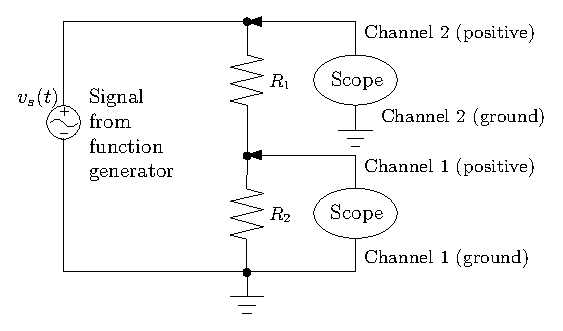
\includegraphics[width=0.45\textwidth]{figs/ipe/lab5/figure4-scopeCircuit}
    \caption{AC voltage applied to two resistors connected in series.}
    \label{fig:figure4-scopeCircuit}
\end{figure}
%
Note that $v_1(t)$ and $v_2(t)$ denote the voltage (time-varying) across resistors $R_1$ and $R_2,$ respectively. Measure the voltages $v_1(t)$ and $v_2(t)$ using the Channel~1 and Channel~2 probes. Make sure to follow  the connections shown in Figure~\ref{fig:figure4-scopeCircuit}.  Record your measurements in the following table, where  $V_{1,\text{pp}}$ and $V_{2,\text{pp}}$ denote the peak-to-peak voltages across the resistors $R_1$ and $R_2,$ respectively. 

  \begin{center}
    \begin{tabular}{p{2.5cm}|p{3.0cm}|p{2.5cm}|p{2.5cm}|}
      \toprule
           & Generated voltage (peak-to-peak) & Voltage across $R_1,~(V_{1,\text{pp}})$& Voltage across $R_2,~(V_{1,\text{pp}})$\\
      \toprule
      Computed & $1.0~[\volt]_{\text{pp}}$ & &\\      % all peak-to-peak voltage      
      \hline
      Measured & & &\\
      \bottomrule
    \end{tabular}    
  \end{center}
  
  \begin{mdframed}[roundcorner=10pt,backgroundcolor=yellow!5]
    Note that the time-varying voltage across the resistor $R_1,~v_1(t),$ can be obtained by subtracting the time-varying voltage across the resistor $R_2,~v_2(t),$ from the source voltage $v_s(t).$ You are required to use the ``MATH MENU'' of the oscilloscope to perform the subtraction operation to find $v_1(t).$
  \end{mdframed}
   
\end{enumerate}

\subsection{Part~2}
\label{sec:part2}
\begin{enumerate}
\item Use the capacitance meter provided in the laboratory to measure the value of the capacitor used to construct the circuit shown in Figure~\ref{fig:figure5-capacitorCircuit} for an ideal capacitance of $C = 1000~[\pico\farad],$ and then complete the following table.

  \begin{center}
    \begin{tabular}{c|c|c}
      \toprule
      Capacitor &  Ideal & Measured\\
      \toprule
      $C$ & $\ldots$ & $\ldots$\\   %|| R_1 = 
      \bottomrule
    \end{tabular}    
  \end{center}



\item Using the function generator under open-circuit conditions, generate a square wave of amplitude $4.0~[\volt]$ (peak-to-peak) with a frequency of $100~[\kilo\hertz].$

\item Use the oscilloscope to measure the rise time $t_r,$ fall time $t_f,$ period $T,$ pulse width $t_w,$ and percent duty cycle. Record all your measurements in the following table. %
%
  %
  \begin{center}
   \begin{tabular}{|c|c|}
    \toprule
    Quantity & Measured\\
    \toprule
     $t_r$ & \\
     \hline
     $t_f$ & \\
     \hline
     $T$ & \\
     \hline
     $t_w$ & \\
     \hline
     \% Duty cycle & \\     
    \bottomrule
   \end{tabular}    
  \end{center}
   %  

\item Construct the circuit shown in Figure~\ref{fig:figure5-capacitorCircuit}, where $v_s(t)$ is the square wave signal that is generated from the function generator in the previous step. 
%
\begin{figure}
  \centering
  \begin{circuitikz}[american voltages]
    \draw
    (0,0) to[sV,v<=$v_s(t)$,*-,fill=green!50](0,3*\smgrid) --(4*\smgrid,3*\smgrid) to[C,l=$C$] (4*\smgrid,0)--(0,0)node[ground]{};
  \end{circuitikz}
    % 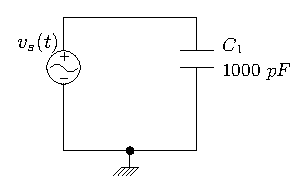
\includegraphics[width=0.3\textwidth]{figs/ipe/lab5/figure5-capacitorCircuit}
    \caption{AC voltage applied to a capacitor.}
    \label{fig:figure5-capacitorCircuit}
\end{figure}
%
  
  
\item  Use the oscilloscope to measure the new rise time and fall time of the pulse generated across the  capacitor. Record all of your measurements in the table below:

    %
  \begin{center}
   \begin{tabular}{|c|c|}
    \toprule
    Quantity & Measured value\\
    \toprule
     $t_r$ & \\
     \hline
     $t_f$ & \\
    \bottomrule
   \end{tabular}    
  \end{center}
   %  

  

 \end{enumerate}


%%% Local Variables:
%%% mode: latex
%%% TeX-master: "../../labBookMechatronics-V2"
%%% End:
